\section{Applying \textit{nETL}}
Using the \textit{nETL} application, lines from the flat data files (CSV files) were extracted in batches of between 10 000 rows and 50 000 rows at at time and loaded into CouchDB. Data-transformation and cleansing, including translating data from tabular format to JSON format, filtering rows, and white-listing attributes was performed as part of this ETL process.

The difference between data in a tabular format (such as a CSV) compared to JSON documents is that every JSON document (row from a CSV) needs both attribute and value information, whereas in visual tables, attributes are specified once as an ordered list once. Rows then consist of ordered values relatable to the value of the attributes list at the corresponding index. Visually (i.e. when working on an Excel file), such association is trivial. JSON documents comprise a list of unordered \textless key:value \textgreater pairs as stipulated in \cite{rfc7159} necessitating the need for a computerized transformation process. Transforming CSV data into JSON data requires maintaining a list of attribute names, iterating through rows and applying those attribute names to values in those rows. The CREATE\_OBJ\_FIELD \textit{nETL} module was composed for this task, the code of which is available in the appendix (\ref{netl-trans-create-obj-field}). A representation of each entity as a JSON object is shown in \ref{tbl-json-examples}.

A batch of data extracted from the CSV files comprised a list of rows (a row comprised a list of values), each of which were individually transformed into JSON documents in this way and stored as a list of documents. This list was then transformed several times and eventually loaded into CouchDB as a list of JSON documents. The source code for \textit{nETL} module responsible for extracting CSV lines is shown in the appendix at \ref{netl-extract-flatfile}, and the source code for the module used to load the data into CouchDB is shown in the appendix at \ref{net-load-couchdb}. Extracting values from a CSV was trickier than anticipated due to surprising variation in answers to the question "What is a CSV?". Variations in CSV formatting result in complexities with delimiting values; a 3rd party CSV-parsing library was used for this task.

The FU data was filtered on two attributes: \textit{Career} with the values "UGRD", "First Year", "Second Year" and "Third Year" accepted, and \textit{Citizenship Residency} with the values "SA Citizen", "Permanent Resident", "C" and "P" accepted. Sakai course grades were filtered on four attributes: \textit{RegCareer} with the value "UGRD" accepted, \textit{Course} with only specific courses accepted (dependent on the analysis), \textit{CourseCareer} with the value "UGRD" accepted, and \textit{CourseSuffix} with the values "F" (semester 1), "S" (semester 2), "H" (single semester course over whole year), and "W" (whole year course) accepted. Sakai events were filtered on the the attribute \textit{event\_id}, with only the value "281" accepted (corresponding to presence events). Filtering was performed by the \textit{nETL} application by the FILTER module, with source code shown in the appendix \ref{netl-trans-filter}.

Following filtering, a white-listing transformation was applied to reduce the number of attributes/document where those attributes were superfluous. In the case of the FU data, no white-listing was needed since unnecessary columns had already been removed when the flat files were manually aggregated in Excel. Grade data was white-listed extensively since only the \textit{Percent} field was really of interest in this study. White-listing was also performed by the \textit{nETL} application; code for the WHITELIST module is shown in the appendix \ref{netl-trans-whitelist}.

A further transformation was applied to all JSON documents within the \textit{nETL} application; an attribute "type\_" was added to each document to identify documents as conceptually belonging to a specific entity (an FU row, a Sakai Grade row, or a Sakai Event row). This was achieved via the CREATE\_OBJ\_FIELD module shown in the appendix \ref{netl-trans-create-obj-field}.

In addition to data transformations applied suring the ETL process by \textit{nETL}, two fields - \textit{Percent} in the grade data and all the percentage fields in the FU data - had inconsistent data types. These fields need to be analyzed as numerical values (i.e. percentages) but were exported as a mixture of percentages, symbols, and abbreviated statuses. These fields were normalized during the MapReduce process discussed later in this project. A description of the different values that needed to be normalized in the Grade data is shown in \ref{tbl-sakai-grades-percent}, with numerical equivalents applied based on estimates of circumstance. Translation of the FU data involved a straight conversion of symbols to numerical numbers ("A" was translated to "80", "B" was translated to "70", etc.).

Achieved via a combination of filtering and white-listing in \textit{nETL}, and further scrubbing in the MapReduce functions, the resultant datasets used for analysis, after scrubbing, filtering, etc. include: 1) benchmarks of undergraduate students that registered for UCT in 2014,2015,2016. 2) Undergraduate course results in 2014, 2015, 2016 for courses that ran in the first semester, second semester, or during the normal school year. 3) A count of 'presence' events for students in 2016 on the Sakai LMS.




Producing a dataset suitable for analysis involves the workflow specified in \ref{analysis-workflow}. The workflow involves configuration of \textit{nETL} tasks to load data from CSVs into CouchDB, authoring of a CouchDB design doc, including a view function (MapReduce) and a list function, asking CouchDB to build the index, retrieving the indexed result via the list function specified in the design document and working with the joined dataset in Excel.

In terms of defining MapReduce tasks, the map function is always user-defined, whereas a built-in reduce function (\_stats) is always used. The built-in reduce function are implemented within the main Erlang process, which according to the documentation offers a performance boost since the IO transfer cost between the Erlang process and the view engine (couchjs.exe by default) is negated. Working on a Windows machine the IO cost is apparently exaggerated (see the slack correspondence with Jan Lehnardt in appendix \ref{slack-1-nov}) due to the difference between Unix-based and Windows kernel implementations.

Analyses are conducted in an iterative fashion; with each iteration an increasing volume of data is handled so as to gain insight into the viability of handling varying amounts of data in CouchDB. Data volume is controlled by the number of courses analyses (more courses taken into account results in higher volumes of data), And the number of entities joined together (grades \& FU data vs grades, FU data, \& Sakai usage). Results are discussed in terms of the insights into business domain (EDM) as well as the effectiveness of the data-mining approach. Runtime results of \textit{nETL}, CouchDB indexing times, database/index storage footprints are shown in Table \ref{performance-analysis}.

\begin{figure}[ht]
    \centering
    \begin{mdframed}
        \centering
        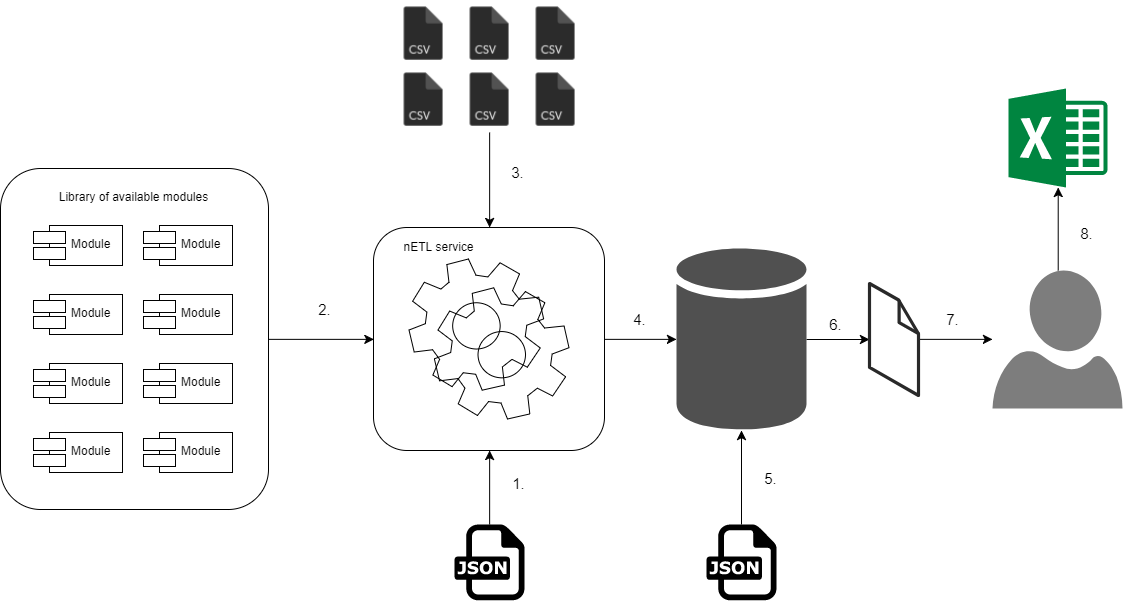
\includegraphics[scale=0.35]{./resources/figures/analysis-workflow.png}
    \end{mdframed}
    \caption[Analysis Workflow]{\textbf{Figure \ref{analysis-workflow}: Workflow to perform an analysis.}1) User creates a configuration file (JSON) that is loaded into the running \textit{\_nETL} service. This configuration includes instructions on which CSVs to load, which modules should be loaded to process the CSVs, and configurations for the modules. 2) Modules are loaded from a library of available modules into the \textit{\_nETL} service. 3) CSVs are loaded into the service, and transformations are applied to the CSV data as specified by the configuration in (1). 4) Data from the CSVs is loaded into CouchDB; this is also achieved via a module specified in (1). 5) A user creates a CouchDB design document, specifying the MapReduce functions, and a List function. 6) The user asks CouchDB to produce the view index as specified by the design document in (5). 7) The user retrieves the data from the view index using the list function specified in (5). 8) The user then loads the resultant CSV into Excel to produce useful metrics.}
    \label{analysis-workflow}
\end{figure}





\begin{table}[h]
    \begin{threeparttable}
        \textbf{Table \ref{performance-analysis}}\par\medskip\par\medskip
        \caption[Software performance analysis]{Running time analysis of \textit{nETL} tasks and CouchDB MapReduce indexing}
        \label{performance-analysis}
        \begin{tabularx}{\textwidth}{>{\hsize=1\hsize}Y>{\hsize=1\hsize}X>{\hsize=1\hsize}X>{\hsize=1\hsize}X>{\hsize=1\hsize}X}
            \toprule
            \mC{c}{}                                               & \mC{c}{Run 1} & \mC{c}{Run 2} & \mC{c}{Run 3} & \mC{c}{Run 4} \\
            \midrule
            Demographic lines extracted                            & 12 219        & 12 219        & 12 219        &               \\
            Demographic lines loaded                               & 1 381         & 9 874         & 595           &               \\
            Demographic task time (sec)\tnote{\textsuperscript{1}} & 2.488         & 3.114         & 6.755         &               \\
            Grade lines extracted                                  & 513 872       & 513 872       & 513 872       &               \\
            Grade lines loaded                                     & 1 891         & 79 849        & 738           &               \\
            Grade task time (sec)\tnote{\textsuperscript{1}}       & 37.684        & 42.001        & 97.221        &               \\
            Events lines extracted                                 & -             & -             & 44 420 508    &               \\
            Events lines loaded                                    & -             & -             & 661 555       &               \\
            Events task time (sec)\tnote{\textsuperscript{1}}      & -             & -             & 2 225.44      &               \\
            CouchDB footprint (MB)\tnote{\textsuperscript{2}}      & 0.9           & 23.2          & 172.1         &               \\
            View calculation time (sec)\tnote{\textsuperscript{3}} & 0.685         & 49.042        & 340.413       &               \\
            View size (MB)                                         & 0.813         & 143           & 521           &               \\
            \bottomrule
        \end{tabularx}
        \scriptsize
        \begin{tablenotes}
            \item[\textsuperscript{1}]Tasks are run asynchronously, so time taken includes processing of other tasks in this run. Task run times are printed out to the log
            \item[\textsuperscript{2}]This is representative of the amount of data processed by \textit{nETL}
            \item[\textsuperscript{3}]CouchDB views are calculated per shard. By default a database contains 8 shards (even in single node mode). The log file shows start and end times of view calculations for each shard, the time is taken as time the first shard starts indexing, to the time the last shard stops indexing.
        \end{tablenotes}
    \end{threeparttable}
\end{table}

todo:

Hi Sonia.

I’m looking at the two approaches to using MapReduce to aggregate data across different entities in CouchDB.

A bit about how view are produced in CouchDB:
CouchDB iterates through the docs, and runs the map function on every document, which the user configures to ‘emit’ values. For my function, the emitted value is a tuple with 11 indexes, with every value initialized at 0. So it’s this: [0,0,0,0,0,0,0,0,0,0,0]. Then depending on the document being processed by the map function, values at different indexes are changed.

i.e. if the document being processed by the map function is a ‘grade’ document, then the map function adjusts the value tuple to emit the grade percent – i.e. [percent, 0,0,0,0,0,0,0,0,0,0]. Or if the document is of type ‘demographic’, the map function changes the values at indexes 2 through 9 and emits the value: [0, x,x,x,x,x,x,x,x, 0, 0]. If the document is of type ‘event’, then the map function alters the value at indexes 9 and 10. i.e. [0,0,0,0,0,0,0,0, s1Event, s2Event] (s1Event is 1 for first semester event, or 0 for second semester, etc.).

And as you recommended, the keys are always emitted as [student id, course, year] for grade document, [student id, ‘a’, 1] for demographic documents, and [student id, ‘a’, year] for event documents.

But then I can never group the different document types for a student id. Instead I’m guaranteed that all documents for a single student are ‘next’ to each other and I can join them from iteration as a result. i.e. this is the result of the map function for a single student for 2 courses

    [smtzac002, ‘a’, 1]: [0, b1, b2, b3, b4, b5, b6, b7, b8, 0, 0]
[smtzac002, ‘a’, 2016]: [0, 0, 0, 0, 0, 0, 0, 0, 0, 1, 0]
[smtzac002, ‘a’, 2016]: [0, 0, 0, 0, 0, 0, 0, 0, 0, 1, 0]
[smtzac002, ‘a’, 2016]: [0, 0, 0, 0, 0, 0, 0, 0, 0, 0, 1]
[smtzac002, ‘a’, 2016]: [0, 0, 0, 0, 0, 0, 0, 0, 0, 0, 1]
[smtzac002, ‘a’, 2016]: [0, 0, 0, 0, 0, 0, 0, 0, 0, 0, 1]
[smtzac002, ‘a’, 2016]: [0, 0, 0, 0, 0, 0, 0, 0, 0, 1, 0]
[smtzac002, ‘CSC1015F’, 2016]: [98, 0, 0, 0, 0, 0, 0, 0, 0, 0, 0]
[smtzac002, ‘MAM100F, 2016]: [94, 0, 0, 0, 0, 0, 0, 0, 0, 0, 0]

Then the reduce function is only necessary to aggregate the event data (which will all have the same key). The result is something like this:

[smtzac002, ‘a’, 1]: [0, b1, b2, b3, b4, b5, b6, b7, b8, 0, 0]
[smtzac002, ‘a’, 2016]: [0, 0, 0, 0, 0, 0, 0, 0, 0, 3, 3]
[smtzac002, ‘CSC1015F’, 2016]: [98, 0, 0, 0, 0, 0, 0, 0, 0, 0, 0]
[smtzac002, ‘MAM100F, 2016]: [94, 0, 0, 0, 0, 0, 0, 0, 0, 0, 0]

(although the structure of the reduce output is a little different to this, the information is the same)

Then the actual aggregation is done on retrieval. So it would be better to do the actual aggregation in nETL then.

Is that ok? But this means that the importance of the reduce function is greatly diminished. So effectively I’m using CouchDB to order the information in the CSV, and nothing more really…

Alternatively, what I did was this:
[smtzac002, ‘x’, y]: [0, b1, b2, b3, b4, b5, b6, b7, b8, 0, 0] // this document is emitted twice: where x = CSC1015F, and then when x = MAM100F. y = 2016 (since only one year is analyzed)
[smtzac002, ‘x’, 2016]: [0, 0, 0, 0, 0, 0, 0, 0, 0, 1, 0] // emitted for x = CSC1015F and x = MAM100F
    [smtzac002, ‘x’, 2016]: [0, 0, 0, 0, 0, 0, 0, 0, 0, 1, 0] // emitted for x = CSC1015F and x = MAM100F
    [smtzac002, ‘x’, 2016]: [0, 0, 0, 0, 0, 0, 0, 0, 0, 0, 1] // emitted for x = CSC1015F and x = MAM100F
    [smtzac002, ‘x’, 2016]: [0, 0, 0, 0, 0, 0, 0, 0, 0, 0, 1] // emitted for x = CSC1015F and x = MAM100F
    [smtzac002, ‘x’, 2016]: [0, 0, 0, 0, 0, 0, 0, 0, 0, 0, 1] // emitted for x = CSC1015F and x = MAM100F
    [smtzac002, ‘x’, 2016]: [0, 0, 0, 0, 0, 0, 0, 0, 0, 1, 0] // emitted for x = CSC1015F and x = MAM100F
    [smtzac002, ‘CSC1015F’, 2016]: [98, 0, 0, 0, 0, 0, 0, 0, 0, 0, 0] // emitted once
    [smtzac002, ‘MAM100F, 2016]: [94, 0, 0, 0, 0, 0, 0, 0, 0, 0, 0] // emitted once


So then the result of the reduce function is an aggregation already. BUT. If I am analyzing 40 courses, then every single event is emitted 40 times. And if I were analyzing multiple years, then every event would be emitted 40 times for each year (so 120 times for 3 years). Obviously this is not scalable.

Should I include the fact that I tried this approach in the write up? It seems like more a mistake than anything else in hindsite. I would prefer to just write up the steps to creating a correct and concise result.
